\chapter{Casi d'uso}\label{casi-d-uso}
\section{Attori}

Si richiama alla sezione relativa, \ref{attori} nel capitolo relativo alle user stories.

\section{Sistema di autenticazione}

Il sistema di autenticazione si occupa di gestire gli account degli utenti, di autenticarli e di autorizzarli a compiere determinate azioni.

\paragraph{Obiettivo} Il sistema di autenticazione si propone come goal principale quello di offrire all'utente non autenticato la possibilità di autenticarsi, questa condizione viene poi utilizzata come precondizione in molti degli altri sistemi e casi d'uso.

\section{UC01 - Login}

%Una breve descrizione dello use case

\subsection{Attore}
\subsection{Precondizioni}
\subsection{Post-condizioni}
\subsection{Scenario principale}
\subsection{Scenario alternativo}

\subsection{UC02 - Visualizzazione del messaggio d'errore autenticazione}

\paragraph{Attore primario} L'attore primario è l'utente non autenticato.

\paragraph{Intenzione in contesto} L'attore primario desidera vedere se le credenziali che ha inserito per autenticarsi hanno problemi di qualche sorta.

\section{Sistema di manutenzione}

\section{Sistema di coordinamento}

%lista use-cases
\section{UC02 - Visualizzazione lista aree}\label{uc:02}

\paragraph{Intenzione in contesto} L'attore primario vuole vedere una lista delle varie aree di illuminazione ed il loro stato.

\paragraph{Attore primario} L'attore primario sono l'utente gestore e manutentore.

\paragraph{Precondizioni} L'attore primario è autenticato ed autorizzato dal sistema.

\paragraph{Postcondizioni} L'attore primario vede la lista delle aree.

\paragraph{Scenario principale}

\begin{enumerate}
    \item L'utente richiede la visualizzazione della lista delle aree;
    \item il sistema fornisce la lista delle aree presenti nel sistema.
\end{enumerate}

\begin{figure}[h]
    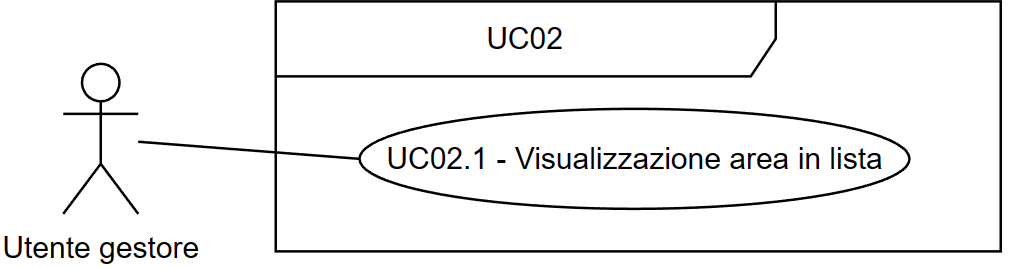
\includegraphics[width=\textwidth]{contenuti/img/casi_uso_grafici-uc02.png}
    \caption{Dettaglio dell'UC02}
    \label{fig:uc02}
\end{figure}

\subsection{UC02.1 Visualizzazione area in lista}
\paragraph{Intenzione in contesto} L'attore primario vuole visualizzare una singola area.

\paragraph{Attore primario} L'attore primario è l'utente gestore.
\paragraph{Precondizioni} L'attore primario è riconosciuto ed autorizzato dal sistema.
\paragraph{Postcondizioni} L'attore primario visualizza la singola area desiderata, in particolare le informazioni relative a \hyperref[uc:02.1.1]{UC02.1.1} e \hyperref[uc:02.1.2]{UC02.1.2}.

\paragraph{Scenario principale}
\begin{enumerate}
    \item L'utente richiede di visualizzare una singola area;
    \item l'utente visualizza la singola area desiderata.
\end{enumerate}

\begin{figure}[h]
    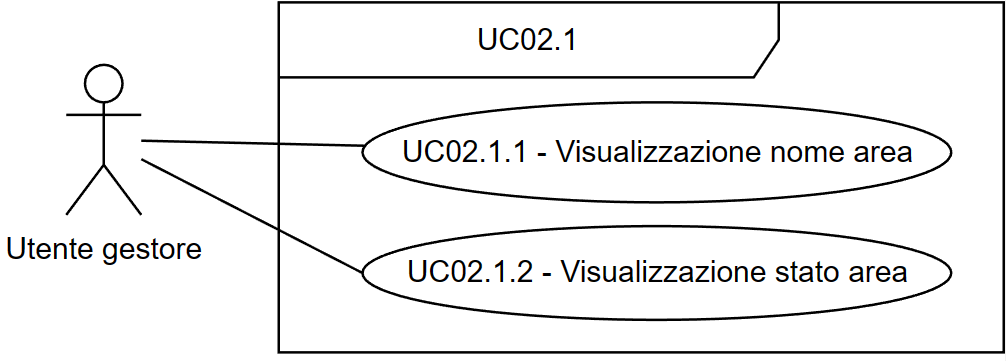
\includegraphics[width=\textwidth]{contenuti/img/casi_uso_grafici-uc02.1.png}
    \caption{Dettaglio dell'UC02.1}
    \label{fig:uc02.1}
\end{figure}

\subsection{UC02.1.1 - Visualizzazione nome area}\label{uc:02.1.1}

\paragraph{Intenzione in contesto} L'attore primario vuole visualizzare il nome dell'area.
\paragraph{Attore primario} L'attore primario è o l'utente gestore o l'utente manutentore.
\paragraph{Precondizioni} L'attore primario è autenticato ed autorizzato dal sistema.
\paragraph{Post-condizioni} L'attore primario visualizza il nome dell'area.
\paragraph{Scenario principale}
\begin{enumerate}
    \item L'attore primario richiede al sistema di visualizzare il nome dell'area;
    \item il nome dell'area è stato visualizzato.
\end{enumerate}

\subsection{UC02.1.2 - Visualizzazione stato area}\label{uc:02.1.2}

\paragraph{Intenzione in contesto} L'attore primario vuole visualizzare lo stato dell'area.
\paragraph{Attore primario} L'attore primario è o l'utente gestore manutentore.
\paragraph{Precondizioni} L'attore primario è autenticato ed autorizzato dal sistema.
\paragraph{Post-condizioni} L'attore primario visualizza lo stato dell'area.
\paragraph{Scenario principale}
\begin{enumerate}
    \item L'attore primario richiede al sistema di visualizzare lo stato dell'area;
    \item lo stato dell'area è stato visualizzato.
\end{enumerate}
\section{UC03 - Visualizzazione dettaglio area}

\paragraph{Attore primario} L'attore primario è l'utente gestore.
\paragraph{Intenzione in contesto} L'attore primario vuole vedere i dettagli specifici di una determinata area di illuminazione. Di questi vuole vederne cose come: stato di accensione, livelli di luminosità impostata.

\paragraph{Precondizioni} L'attore primario è riconosciuto ed autorizzato dal sistema.

\paragraph{Postocondizioni} L'attore primario vede i dettagli e le informazioni sull'area specifica a cui è interessato.

\paragraph{Scenario principale}

\begin{enumerate}
    \item L'utente ha in mente quale area visualizzare
    \item l'utente richiede di visualizzare il dettaglio dell'area;
    \item il sistema fornisce i dettagli relativi all'area scelta.
\end{enumerate}
\section{UC04 - Apertura ticket di guasto}

\paragraph{Descrizione:}
Come \textit{attore principale}(utente gestore/sensore di guasti) desidero aprire un ticket di assistenza in caso di guasto ad un impianto di illuminazione.

\paragraph{Attori principali:}
\begin{itemize}
    \item Utente gestore;
    \item Sensore guasti.
\end{itemize}

\paragraph{Attori secondari:}
\begin{itemize}
    \item Sistema ticketing.
\end{itemize}

\paragraph{Precondizioni:}
L'utente gestore è loggato, e vuole aprire un ticket di guasto.

\paragraph{Post-condizioni:}
Il ticket di guasto è stato aperto nel sistema di ticketing.

\paragraph{Scenario principale:}
\begin{enumerate}
    \item L'attore principale rileva il guasto;
    \item l'attore principale inserisce le informazioni sul guasto;
    \item l'attore principale apre il ticket con le informazione inserite;
    \item il sistema di ticketing riceve le informazioni e conferma l'apertura del ticket.
\end{enumerate}

\paragraph{Scenario alternativo:}
\begin{itemize}
    \item L'attore principale ha inserito informazioni errate e il sistema mostra un errore;
    \item il sistema di ticketing non risponde e il sistema mostra un errore.
\end{itemize}

\section{UC05 - Visualizzazione dettaglio lampione}\label{uc:05}
\paragraph{Attore primario} L'attore primario è l'utente gestore.
\paragraph{Intenzione in contesto} L'attore primario vuole vedere i dettagli di un lampione, di questo vuole conoscerne lo stato.
\paragraph{Precondizioni}L'attore primario è riconosciuto ed autorizzato dal sistema.
\paragraph{Postcondizioni} L'attore primario visualizza i dettagli e le informazioni su uno specifico lampione.
\paragraph{Scenario principale}
\begin{enumerate}
    \item L'utente richiede di visualizzare i dettagli di uno specifico lampione;
    \item l'utente visualizza i dettagli dello specifico lampione.
\end{enumerate}
\section{UC06 - Aggiunta singolo lampione}

%Una breve descrizione dello use case
\paragraph{Descrizione:}
Come utente installatore/manutentore, voglio aggiungere un singolo lampione al sistema.

\subsection{Attore principale:}
Utente installatore/manutentore.

\subsection{Precondizioni:}
L'utente installatore/manutentore vuole aggiungere al sistema un nuovo lampione.

\subsection{Post-condizioni:}
Il lampione è stato aggiunto al sistema.

\subsection{Scenario principale:}
\begin{enumerate}
    \item L'utente installatore/manutentore inserisce i dati relativi al nuovo lampione;
    \item Il nuovo lampione viene aggiunto al sistema.
\end{enumerate}

\subsection{Scenario alternativo:}
\begin{enumerate}
    \item L'utente installatore/manutentore inserisce valori non ammissibili e il sistema ritorna un errore.
\end{enumerate}
\section{UC07 - Visualizzazione lista ticket di guasto}\label{uc:07}
\paragraph{Intenzione in contesto} L'attore primario desidera la lista dei ticket di guasto presenti nel sistema.

\paragraph{Attore primario} L'attore primario è o l'utente gestore o l'utente manutentore.
\paragraph{Precondizioni} L'attore primario è autenticato ed autorizzato dal sistema.
\paragraph{Post-condizioni} L'attore primario visualizza la lista dei ticket di guasto.
\paragraph{Scenario principale}
\begin{enumerate}
    \item L'attore primario richiede al sistema la lista dei ticket di guasto;
    \item la lista è stata visualizzata.
\end{enumerate}

\begin{figure}[h]
    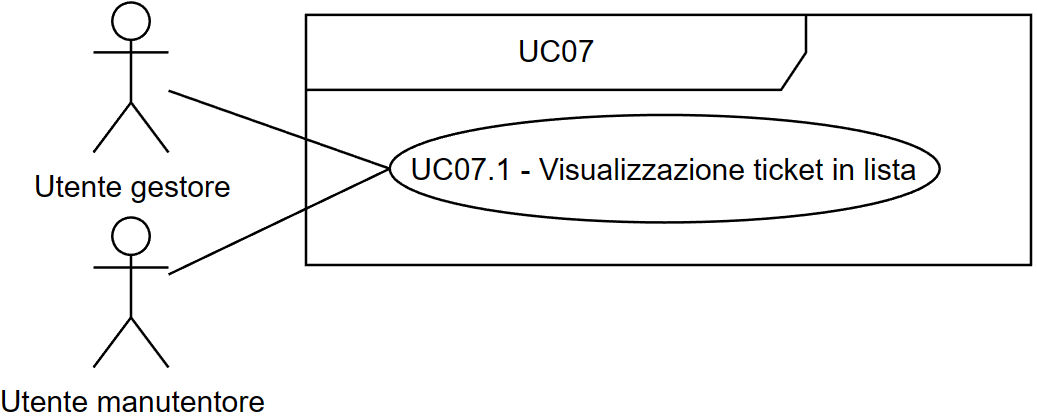
\includegraphics[width=\textwidth]{contenuti/img/casi_uso_grafici-uc07.png}
    \caption{UC7 in dettaglio}
    \label{fig:uc07}
\end{figure}

\subsection{UC07.1 - Visualizzazione ticket in lista}\label{uc:07.1}
\paragraph{Intenzione in contesto} L'attore primario vuole visualizzare il singolo ticket parte della lista.
\paragraph{Attore primario} L'attore primario è o l'utente gestore o l'utente manutentore.
\paragraph{Precondizioni} L'attore primario è autenticato ed autorizzato dal sistema.
\paragraph{Post-condizioni} L'attore primario visualizza il singolo ticket.
\paragraph{Scenario principale}
\begin{enumerate}
    \item L'attore primario richiede al sistema di visualizzare il singolo ticket in lista;
    \item il ticket è stato visualizzato.
\end{enumerate}

\begin{figure}[h]
    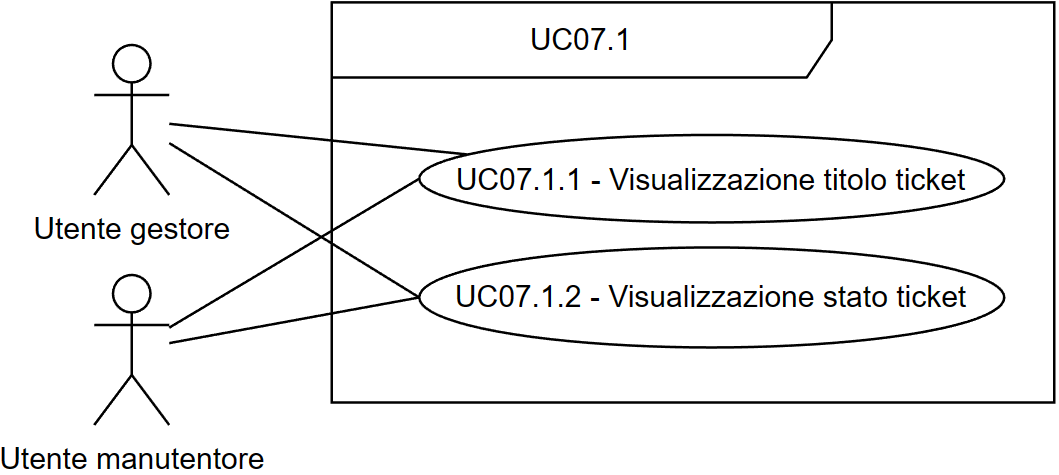
\includegraphics[width=\textwidth]{contenuti/img/casi_uso_grafici-uc07.1.png}
    \caption{UC07.1 in dettaglio}
    \label{fig:uc07.1}
\end{figure}

\subsection{UC07.1.1 - Visualizzazione titolo ticket}\label{uc:07.1.1}

\paragraph{Intenzione in contesto} L'attore primario vuole visualizzare il titolo del ticket;
\paragraph{Attore primario} L'attore primario è o l'utente gestore manutentore.
\paragraph{Precondizioni} L'attore primario è autenticato ed autorizzato dal sistema.
\paragraph{Post-condizioni} L'attore primario visualizza il titolo del ticket.
\paragraph{Scenario principale}
\begin{enumerate}
    \item L'attore primario richiede al sistema di visualizzare il titolo del ticket;
    \item il titolo del ticket è stato visualizzato.
\end{enumerate}

\subsection{UC07.1.2 - Visualizzazione stato ticket}\label{uc:07.1.2}

\paragraph{Intenzione in contesto} L'attore primario vuole visualizzare lo stato del ticket;
\paragraph{Attore primario} L'attore primario è o l'utente gestore manutentore.
\paragraph{Precondizioni} L'attore primario è autenticato ed autorizzato dal sistema.
\paragraph{Post-condizioni} L'attore primario visualizza lo stato del ticket.
\paragraph{Scenario principale}
\begin{enumerate}
    \item L'attore primario richiede al sistema di visualizzare lo stato del ticket;
    \item lo stato del ticket è stato visualizzato.
\end{enumerate}
\section{UC08 - Visualizzazione dettaglio ticket}\label{uc:08}
\paragraph{Intenzione in contesto} L'attore primario desidera visualizzare la pagina di dettaglio del ticket.

\paragraph{Attore primario} L'attore primario è o l'utente gestore o l'utente manutentore.
\paragraph{Precondizioni} L'attore primario è autenticato ed autorizzato dal sistema.
\paragraph{Post-condizioni} L'attore primario visualizza la pagina di dettaglio dei ticket di guasto.
\paragraph{Scenario principale}
\begin{enumerate}
    \item L'attore primario richiede al sistema la pagina di dettaglio del ticket di guasto;
    \item la pagina di dettaglio del ticket viene visualizzata, in particolare le informazioni relative a \hyperref[uc:08.1]{UC08.1} e \hyperref[uc:08.2]{UC08.2}.
\end{enumerate}

\begin{figure}[h]
    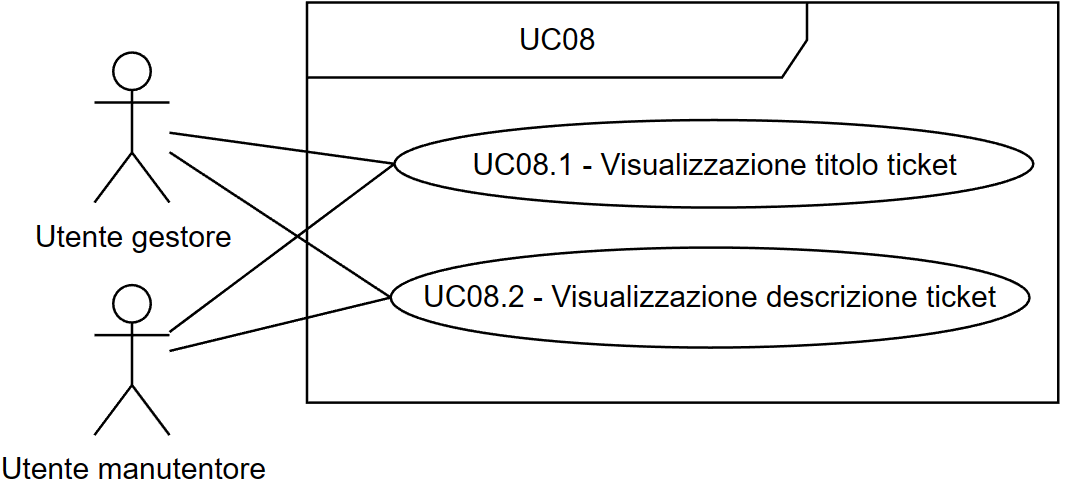
\includegraphics[width=\textwidth]{contenuti/img/casi_uso_grafici-uc08.png}
    \caption{UC08 in dettaglio}
    \label{fig:uc08}
\end{figure}


\subsection{UC08.1 - Visualizzazione titolo ticket}\label{uc:08.1}

\paragraph{Intenzione in contesto} L'attore primario vuole visualizzare il titolo del ticket;
\paragraph{Attore primario} L'attore primario è o l'utente gestore o l'utente manutentore.
\paragraph{Precondizioni} L'attore primario è autenticato ed autorizzato dal sistema.
\paragraph{Post-condizioni} L'attore primario visualizza il titolo del ticket.
\paragraph{Scenario principale}
\begin{enumerate}
    \item L'attore primario richiede al sistema di visualizzare il titolo del ticket;
    \item il titolo del ticket è stato visualizzato.
\end{enumerate}

\subsection{UC08.2 - Visualizzazione descrizione ticket}\label{uc:08.2}

\paragraph{Intenzione in contesto} L'attore primario vuole visualizzare la descrizione testuale del ticket;
\paragraph{Attore primario} L'attore primario è o l'utente gestore o l'utente manutentore.
\paragraph{Precondizioni}  L'attore primario è autenticato ed autorizzato dal sistema.
\paragraph{Post-condizioni} L'attore primario visualizza la descrizione del ticket.
\paragraph{Scenario principale}
\begin{enumerate}
    \item L'attore primario richiede al sistema di visualizzare la descrizione del ticket;
    \item la descrizione del ticket è stata visualizzata.
\end{enumerate}
\section{UC09 - Inserimento sensore a sistema}

\paragraph{Attore primario} L'attore primario è l'utente manutentore
\paragraph{Intenzione in contesto} L'attore primario vuole aggiungere al sistema un sensore che ha appena installato.

\paragraph{Precondizioni} L'attore primario è autenticato ed autorizzato dal sistema.

\paragraph{Postcondizioni} Il sensore è inserito a sistema ed il sistema può gestirne le informazioni.

\paragraph{Scenario principale}

\begin{enumerate}
    \item L'attore principale ha installato fisicamente il sensore;
    \item l'attore principale inserisce i dati del sensore a sistema;
    \item l'attore principale configura il sensore nella giusta area di appartenenza;
    \item Il sensore viene gestito dal sistema ed utilizzato.
\end{enumerate}

\section{UC10 - Aggiunta area al sistema}\label{uc:10}
\paragraph{Intenzione in contesto} L'attore principale vuole aggiungere una nuova area di gestione dell'illuminazione.

\paragraph{Attore principale} L'attore principale è l'utente manutentore.

\paragraph{Precondizioni}
L'utente principale è autenticato ed autorizzato e vuole aggiungere un area di gestione illuminazione al sistema.

\paragraph{Post-condizioni}
Una nuova area di gestione è stata creata.

\paragraph{Scenario principale}
\begin{enumerate}
    \item L'attore principale crea la nuova area di gestione, inserendo i dati dell'area;
    \item L'area di gestione viene creata nel sistema.
\end{enumerate}

